\documentclass[border=6pt]{standalone}
\usepackage{tikz}
\usetikzlibrary{shapes.geometric, arrows.meta, positioning}
\begin{document}
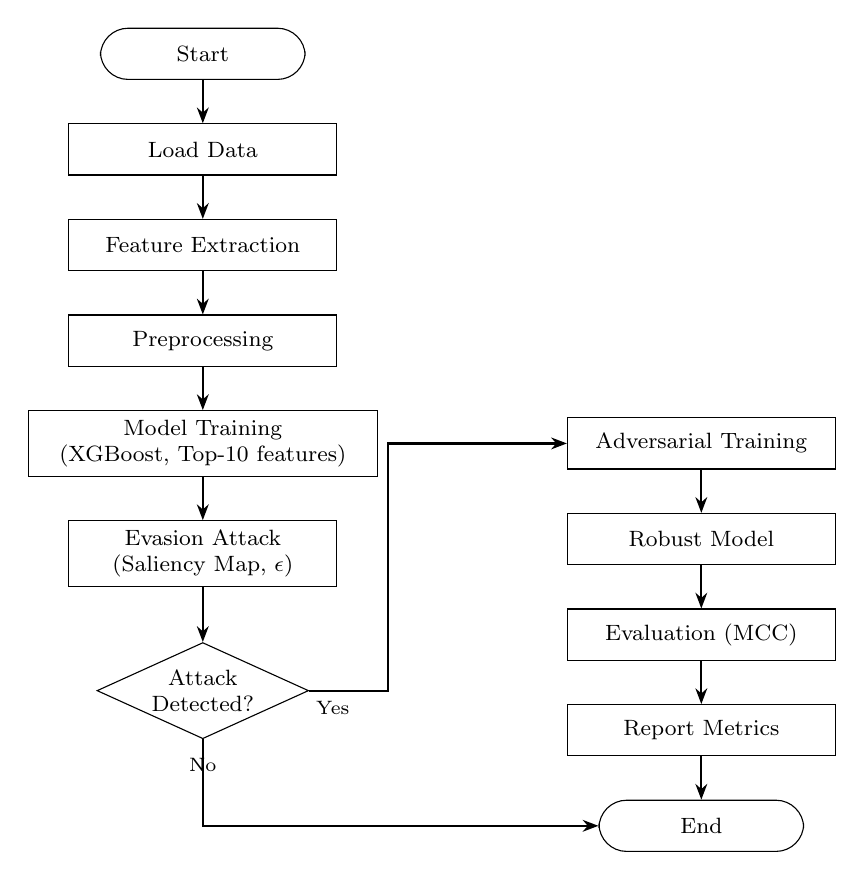
\begin{tikzpicture}[
    node distance=0.55cm,
    every node/.style={font=\footnotesize},
    term/.style={draw, rounded corners=10pt, minimum width=2.6cm, minimum height=0.65cm, align=center},
    proc/.style={draw, minimum width=3.4cm, minimum height=0.65cm, align=center},
    dec/.style={draw, diamond, aspect=2.2, inner sep=1pt, align=center},
    ar/.style={-{Stealth[length=2mm]}, thick}
]
% Left column: backup/detection flow
\node[term] (start) {Start};
\node[proc, below=of start] (upload) {Load Data};
\node[proc, below=of upload] (hash) {Feature Extraction};
\node[proc, below=of hash] (pre) {Preprocessing};
\node[proc, below=of pre, text width=4.2cm] (train) {Model Training\\(XGBoost, Top-10 features)};
\node[proc, below=of train] (attack) {Evasion Attack\\(Saliency Map, $\epsilon$)};
\node[dec, below=0.7cm of attack] (det) {Attack\\Detected?};
% Right column: response flow
\node[proc, right=2.4cm of train] (advtrain) {Adversarial Training};
\node[proc, below=of advtrain] (robust) {Robust Model};
\node[proc, below=of robust] (eval) {Evaluation (MCC)};
\node[proc, below=of eval] (report) {Report Metrics};
\node[term, below=of report] (finish) {End};
% left arrows
\draw[ar] (start) -- (upload);
\draw[ar] (upload) -- (hash);
\draw[ar] (hash) -- (pre);
\draw[ar] (pre) -- (train);
\draw[ar] (train) -- (attack);
\draw[ar] (attack) -- (det);
% Yes -> adversarial training (right column top)
\draw[ar] (det.east) -- node[below, font=\scriptsize, pos=0.3]{Yes} ++(1.0cm,0) |- (advtrain.west);
% right arrows
\draw[ar] (advtrain) -- (robust);
\draw[ar] (robust) -- (eval);
\draw[ar] (eval) -- (report);
\draw[ar] (report) -- (finish);
% No -> straight to End (left edge)
\draw[ar] (det.south) |- node[below, font=\scriptsize, pos=0.05]{No} (finish.west);
\end{tikzpicture}
\end{document}
